% AINTEC 2026 — POSTER ABSTRACT (main poster)
%
% Per the poster CFP: abstract report, at most two double-column pages including
% figures and tables, references excluded; ACM proceedings template; author names
% NOT anonymized. Deadline per the live HotCRP portal: Mon 2026-09-28 8pm EDT =
% Tue 2026-09-29 07:00 Thai (NOT the CFP page's generic 23:59 AoE / 18:59 Thai —
% the portal's own countdown is authoritative for this specific submission).
% The A1 poster itself is only produced if accepted (notification 2026-10-09).
%
% Scope note: the operator / ISP market-structure material was split off on
% 2026-09-24 into a separate poster owned by Kunanont Malayanont. Nothing
% operator-layer belongs in this abstract. See docs/poster/isp/content.md.
%
% Numbers here are the poster-verified set (docs/poster/poster.tex and
% docs/poster/poster_content.md section 3, "Version B" regenerated 9-country
% figures), NOT the paper's 8-country prose numbers. Do not mix the two.
\documentclass[sigconf,nonacm]{acmart}

\usepackage{microtype}
\emergencystretch=2em

\AtBeginDocument{%
  \providecommand\BibTeX{{Bib\TeX}}}

\setcopyright{none}
\copyrightyear{2026}
\acmYear{2026}
\acmDOI{XXXXXXX.XXXXXXX}
\acmConference[AINTEC '26]{Asian Internet Engineering Conference}{2026}{Thailand}
\acmISBN{978-1-4503-XXXX-X/2026/XX}

\settopmatter{printacmref=false, authorsperrow=3}
\renewcommand\footnotetextcopyrightpermission[1]{}

\begin{document}

\title{Beyond Speed Rankings: Application-Layer Broadband Performance
  in Nine Southeast Asian Countries}

\author{Chissanupun Athiwarikanon}
\email{chissanupun.a@ku.th}
\affiliation{%
  \institution{Kasetsart University}
  \city{Bangkok}
  \country{Thailand}
}
\author{Kunanont Malayanont}
\email{kunanont.m@ku.th}
\affiliation{%
  \institution{Kasetsart University}
  \city{Bangkok}
  \country{Thailand}
}
\author{Pakkapon Pattanakul}
\email{pakkapon.p@ku.th}
\affiliation{%
  \institution{Kasetsart University}
  \city{Bangkok}
  \country{Thailand}
}

\renewcommand{\shortauthors}{Athiwarikanon et al.}

\begin{abstract}
Southeast Asian broadband is usually judged by headline speed-index
rankings, which say little about whether real applications work. Thailand
ranked 12th worldwide for fixed broadband in June 2026, yet a 2023 national
consumer survey found 81\% of 2{,}924 respondents reporting connection
problems~\cite{TCC2023}. We analyze 990 million speed tests --- 229.4M
from Ookla Open Data and 760.6M from M-Lab NDT7, Q1 2023 to Q4 2025 ---
across nine countries, and score each country-quarter's median download
speed against the bandwidth requirements of voice, HD video, UHD video and
cloud gaming (bandwidth only; we do not assess latency, and both datasets
are crowdsourced and user-initiated rather than a random sample). Our
preliminary results show that median speeds clear the voice and HD-video
bandwidth bars in every country, every quarter of 2024--2025. That
uniformity collapses at higher tiers. Fixed broadband stratifies sharply by
geography, with a 16$\times$ spread between the strongest and weakest
capital regions, and against the cloud-gaming bandwidth bar the median
reaches 100\% in Singapore but only a peak of 37\% in Indonesia and 31\%
in Myanmar. Work is ongoing on per-province modeling and on peak-hour
behavior.
\end{abstract}

\keywords{Internet measurement, broadband performance, Southeast Asia,
  Ookla, M-Lab NDT7, application requirements}

\maketitle

\section{Motivation}
National broadband quality in Southeast Asia is usually argued from two
sources that disagree with each other: index rankings and user complaints.
Thailand was ranked 12th worldwide for fixed broadband in Ookla's Speedtest
Global Index in June~2026~\cite{OoklaGlobalIndex2026}, while a 2023 survey
by the Thailand Consumer Council found that 81\% of 2{,}924 respondents had
encountered connection problems, mostly slow or dropping
connections~\cite{TCC2023}. A
national mean download speed cannot reconcile those two observations,
because it describes the network rather than the service a user is trying
to run over it.

We therefore ask a different question: \emph{how do Southeast Asian
networks perform against the demands of the applications people actually
use?} Rather than ranking countries by speed, we score every
country-quarter against published bandwidth requirements and report how
close each country's median connection comes to clearing each bar. The mismatch above is not unique
to Thailand, so we run the analysis across nine countries.

\section{Data and Method}
We use two complementary open datasets covering Thailand, Vietnam, Laos,
Myanmar, Cambodia, Indonesia, the Philippines, Malaysia and Singapore, over
twelve quarters (Q1~2023--Q4~2025):

\begin{itemize}
  \item \textbf{Ookla Open Data}~\cite{OoklaOpenData2023} --- 229{,}367{,}221
    tests, published as quarterly tiles of roughly
    600\,m$\times$600\,m, fixed and mobile. Ookla servers sit inside
    access networks and use parallel streams, so these tests
    characterize last-mile capacity.
  \item \textbf{M-Lab NDT7}~\cite{MLabNDT72025} --- 760{,}607{,}387
    single-stream tests to off-net servers, closer to what a single
    streaming or browsing flow observes.
\end{itemize}

Tiles are assigned to first-level administrative provinces by
point-in-polygon against geoBoundaries ADM1~\cite{Runfola2020}; NDT7 points
are joined to the same polygons. Province averages are test-weighted, and we
keep only province-quarters with at least 100 tests and at least 5 tiles.
Tests with non-positive throughput or duration are dropped, and IP
addresses are checked against ip-api.com to exclude hosting/proxy traffic.
Because user-initiated speed tests are a biased sample~\cite{Deng2021}, we
report distributions and success rates rather than treating any single
figure as a population mean. Coverage is uneven: Myanmar is missing 10.7\%
of fixed and 22\% of mobile province-quarters, and some Vietnamese and
Cambodian provinces lack mobile data in low-volume quarters --- gaps we
flag rather than interpolate.

We evaluate four application classes against the thresholds of
L\"ubben and Misfeld~\cite{Lubben2022}: voice (64\,kbps), HD video
streaming (5\,Mbps), UHD video streaming (25\,Mbps) and cloud gaming
(44\,Mbps). \textbf{Success rate} is a country's quarterly median download
speed as a percentage of the application's \emph{download-speed} threshold,
capped at 100\%, reported for the eight quarters Q1~2024--Q4~2025. We
deliberately do not evaluate the 25\,ms latency component of the
cloud-gaming requirement: for six of our nine countries most M-Lab tests
terminate abroad (Thai tests mainly in Singapore and Hong Kong), and only
Singapore, Indonesia and the Philippines are served largely in-country, so
measured round-trip time mostly reflects international transit rather than
domestic access.

\section{Preliminary Results}

\subsection{Median speeds clear the low-bandwidth bars}
The median download speed clears the voice and HD-video bandwidth
thresholds (a 100\% score) in every country, in every quarter of
2024--2025. This holds for the lowest-tier markets in
the set as firmly as for Singapore. Whatever the regional digital divide
consists of, a national median failing to reach 5\,Mbps is not part of it
--- though this says nothing about the tail of individual tests, or about
latency, which we do not evaluate.

\subsection{Fixed broadband stratifies by geography}
\begin{figure}[t]
  \centering
  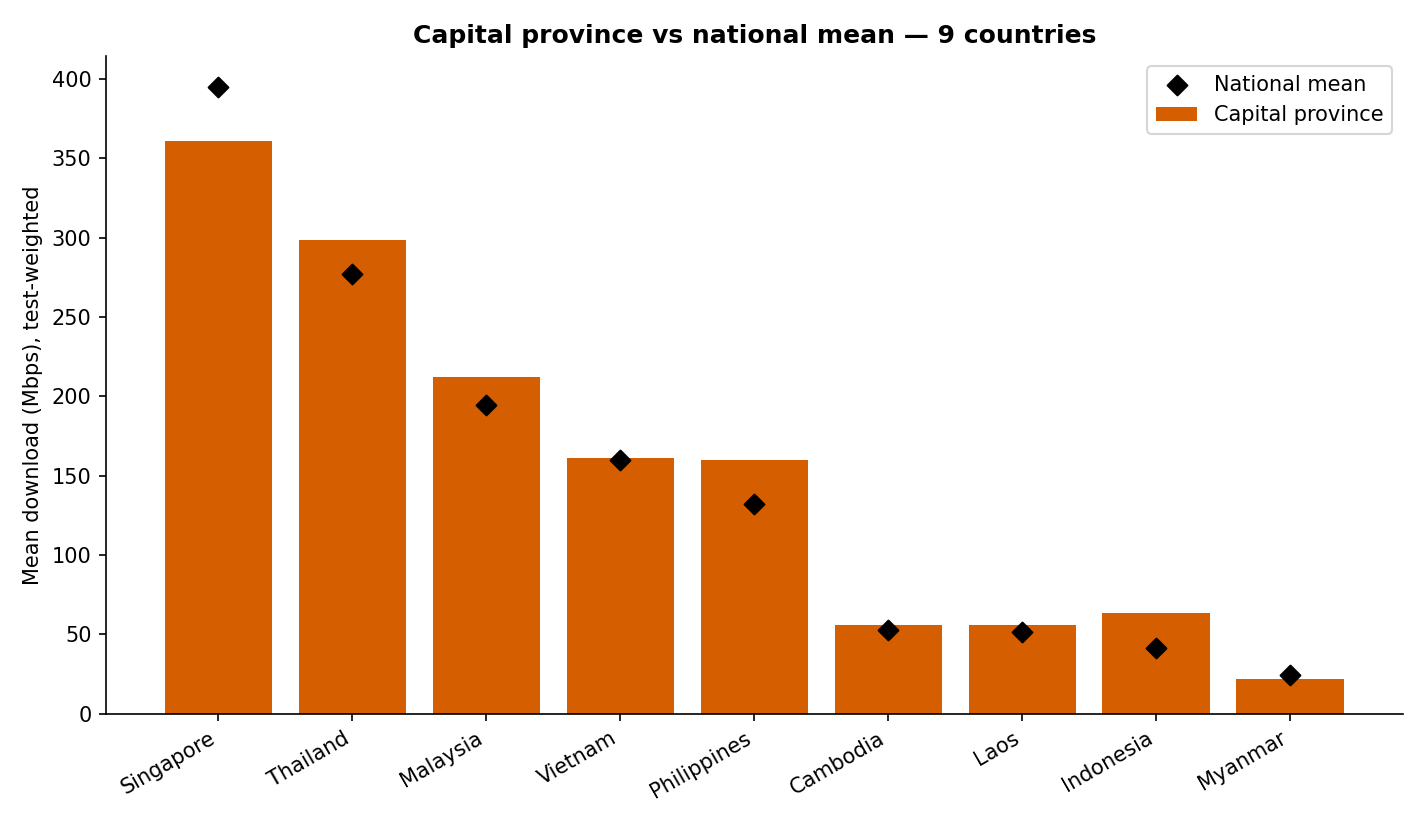
\includegraphics[width=\linewidth]{../../../outputs/ookla/cross_country/03_capital_vs_national.png}
  \caption{Capital province versus national mean download speed, fixed
    broadband, test-weighted, nine countries.}
  \label{fig:capital}
\end{figure}

Most capital regions outperform their own country
(Figure~\ref{fig:capital}): Bangkok reaches 298.8\,Mbps against a national
276.9, Kuala Lumpur 212.3 against 194.8, and Manila NCR 159.6 against
132.0. Singapore and Myanmar are the exceptions: Singapore's Central
Region (361.0) sits \emph{below} its national mean (394.8), as does Yangon
(22.0 against 24.6). The spread between the strongest and weakest capital
region is over 16$\times$ (Singapore's 361.0 against Yangon's 22.0\,Mbps),
a gap that a table of national averages conceals.

The trajectory is also diverging rather than converging. Singapore nearly
doubled its median provincial fixed speed over the period, from roughly 280
to 550\,Mbps, and Thailand grew from roughly 200 to 300. Vietnam
accelerated to join Malaysia above 200\,Mbps. Laos, Cambodia, Indonesia and
Myanmar remained below 60\,Mbps for all three years.

The fixed--mobile gap also varies widely. Fixed broadband exceeds mobile by
3.2$\times$ in Thailand and 2.1$\times$ in Singapore, but the two are near
parity in Malaysia and Indonesia (1.1$\times$), and Myanmar is the only
country in the set where mobile is \emph{faster} than fixed (0.8$\times$)
--- a mobile-first market.

\subsection{Application tiers diverge}
\begin{figure}[t]
  \centering
  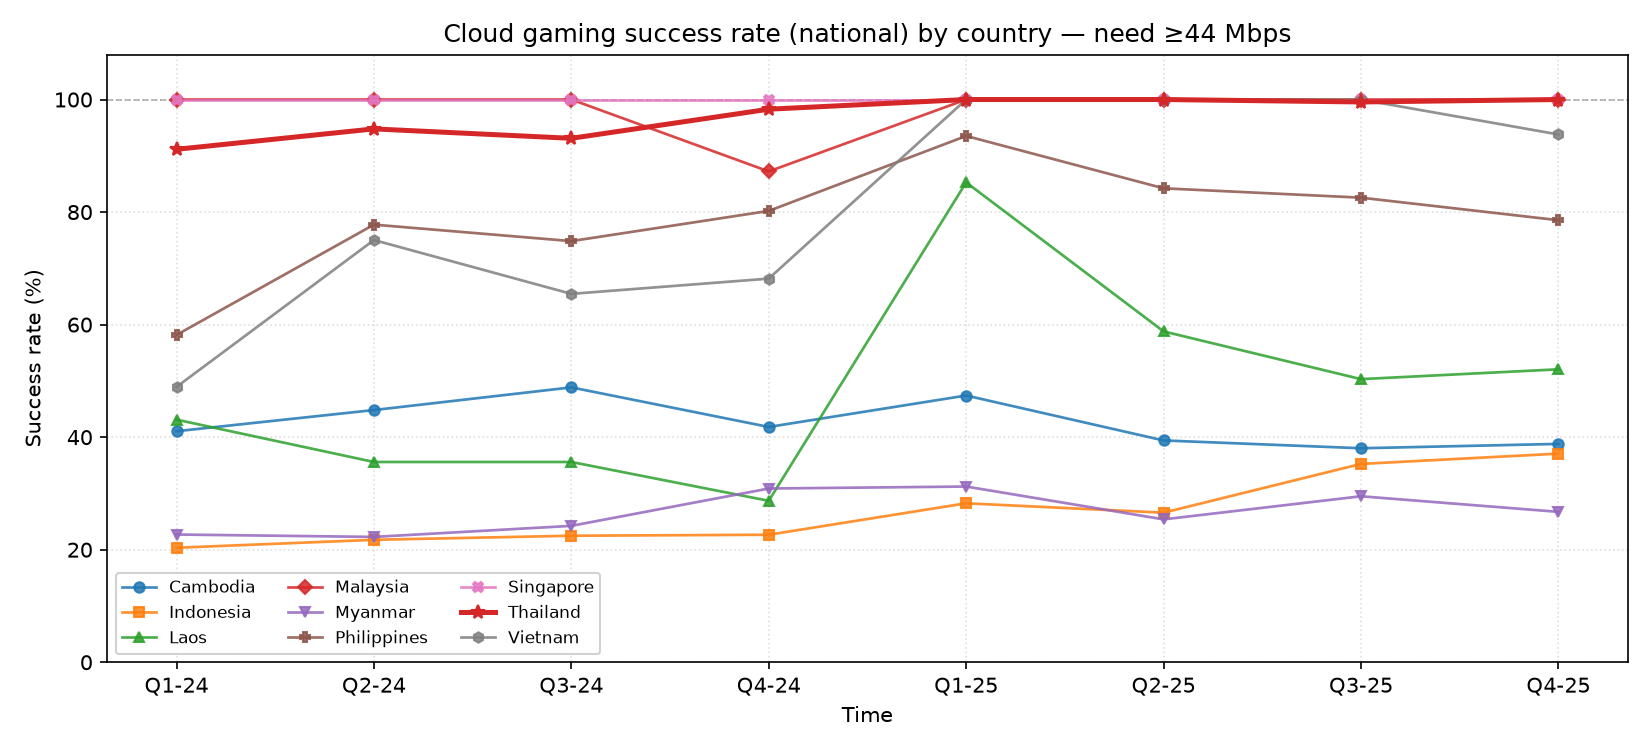
\includegraphics[width=\linewidth]{../../../outputs/app_success_rate_median/fig_cloud_gaming_national.png}
  \caption{Cloud-gaming success rate (median download against the 44\,Mbps
    threshold, capped at 100\%) by country
    and quarter, Q1~2024--Q4~2025.}
  \label{fig:cloudgaming}
\end{figure}

Raising the bar from HD to UHD video separates the region into two groups.
Malaysia, Singapore, Thailand and the Philippines score 100\% at the
25\,Mbps threshold every quarter, as does Vietnam from Q2~2024 (86\% in
Q1). Cambodia ranges from 67\% to 86\%, Indonesia improves from 36\% to
65\%, and Myanmar stays between 39\% and 55\%. Laos is volatile across the full 50--100\%
range, which we attribute to its small measurement volume rather than to
genuine quarter-to-quarter swings in capacity.

Cloud gaming separates them further (Figure~\ref{fig:cloudgaming}).
Singapore's median clears the 44\,Mbps bar in every quarter (100\%), and
Thailand and Malaysia score 87--100\%. The Philippines ranges from 58\% to
94\%, and Vietnam climbs from under 50\% to 94--100\% in 2025. At the other
end, Cambodia reaches only 38--49\%, Laos swings between 29\% and 85\%,
Indonesia peaks at 37\% and Myanmar at 31\% --- meaning their median
download speed reaches barely a third of the cloud-gaming bandwidth
requirement. Networks whose median clears the voice bar
everywhere can still fall far short of what a bandwidth-hungry interactive
application needs.

\section{Ongoing and Future Work}
Three directions are in progress. First, we are fitting province-level
models of speed against economic and density covariates to separate
infrastructure effects from wealth effects. Second, we are extending the
NDT7 analysis to peak-hour behavior, where busy-versus-quiet \emph{ratios}
remain interpretable even though absolute latency is not, given offshore
server placement. Third, we are quantifying the measurement bias introduced
by thin-sample provinces, which currently inflate the apparent performance
of several emerging markets.

The broader argument we wish to discuss at the poster session is that a
speed index answers the wrong question. Basic access across Southeast Asia
is effectively universal; what separates these markets is whether their
networks survive contact with a demanding application, and that distinction
points at different infrastructure investment than a ranking does.

\bibliographystyle{ACM-Reference-Format}
\bibliography{../../paper/references}

\end{document}
